\section{Clases de equivalencia}
\begin{frame}{Concepto de clase}
	Volviendo al ejemplo de las filas. Sabemos que si varias personas tienen la misma edad, entonces forman una fila. Resulta que el conjunto de todos los elementos que están mutuamente relacionados (la fila) cumple ciertas propiedades.
	\begin{enumerate}
		\item Ninguna fila está vacía.
		\item No hay una persona en dos filas diferentes.
		\item Todas las personas están en una fila.
	\end{enumerate}
	A lo que denominamos \emph{fila}, en este caso, es a lo que se le denomina de forma general como \emph{clase de equivalencia}.
\end{frame}
\begin{frame}{Clase de equivalencia}
	\begin{mdefinition}[Clase de equivalencia]
		Sean $ A $ un conjunto, $ \sim\subseteq A^{2} $ una relación de equivalencia y $ a\in A $. Definimos a la \emph{clase de equivalencia} de $ a $ como:
		\[ \bracket{a}\coloneqq\set{b\in A: a\sim b} \]
	\end{mdefinition}
\end{frame}
\begin{frame}
	\begin{exercise}
		Dada la relación de equivalencia de fracciones equivalentes, determine la clase de equivalencia de $ \frac{3}{2} $ y $ \frac{1}{2} $.
	\end{exercise}
\end{frame}
\begin{frame}
	
\end{frame}
\begin{frame}
	\begin{exercise}
		Dada la relación de equivalencia de fracciones equivalentes. Demuestre que si $ n\in\nmath $, entonces:
		\[ \bracket{n} =\set{(nt, t)\in\nmath[2]: t\in\nmath} \]
	\end{exercise}
\end{frame}
\begin{frame}
	
\end{frame}
\begin{frame}
	\begin{exercise}
		Dada la relación de equivalencia de fracciones equivalentes. Demuestre que para cada fracción $ \frac{a}{b} $, su clase de equivalencia es:
		\[ \bracket{\dfrac{a}{b}} =\set{(at, bt)\in\nmath[2]: t\in\nmath} \]
	\end{exercise}
\end{frame}
\begin{frame}
	
\end{frame}
\begin{frame}
	\begin{exercise}
		Dada la relación de equivalencia de módulos, determine la clase de equivalencia de $ 2, 3, 4 $ cuando $ n = 5 $.
	\end{exercise}
\end{frame}
\begin{frame}
	
\end{frame}
\begin{frame}
	\begin{exercise}
		Dada la relación de equivalencia de módulos. Demuestre que para cada $ a\in\zmath $, su clase de equivalencia es:
		\[ \bracket{a} =\set{nk + a\in\zmath: k\in\zmath} \]
	\end{exercise}
\end{frame}
\begin{frame}
	\begin{mtheorem}[Propiedades de las clases de equivalencia]
		\label{thm: clases}
		Sea $ A $ un conjunto, $ \sim\subseteq A^{2} $ y $ a, b\in A $.
		\begin{enumerate}
			\item $ \bracket{a}\neq\varnothing $
			\item $ a\sim b\iff\bracket{a} =\bracket{b} $
			\item $ \bracket{a}\neq\bracket{b}\iff\bracket{a}\cap\bracket{b} =\varnothing $
		\end{enumerate}
	\end{mtheorem}
\end{frame}
\begin{frame}{Demostración}
	\begin{proof}
		\begin{itemize}
			\only{
				\item $ \bracket{a}\neq\varnothing $\\
				Sabemos que $ a\sim a $, por lo tanto la clase de $ a $ tiene al menos como elemento a $ a $. Por lo tanto, $ \bracket{a}\neq\varnothing $
			}<1>
			\only{
				\item $ a\sim b\iff\bracket{a} =\bracket{b} $
				\begin{itemize}
					\item[$ \implies) $] Sea $ w\in\bracket{b} $, entonces $ b\sim w $ y por transitividad $ a\sim w $, es decir que $ w\in\bracket{a} $. Por lo tanto, $ \bracket{b}\subseteq\bracket{a} $.\par 
					Sea $ w\in\bracket{a} $, entonces $ w\sim a $ y por transitividad $ w\sim b $ es decir que $ w\in\bracket{b} $. Por lo tanto, $ \bracket{a}\subseteq\bracket{b} $.\par
					Por lo tanto, $ \bracket{a} =\bracket{b} $.
					\item[$ \impliedby) $] Dado que $ \bracket{a} =\bracket{b} $, entonces claramente $ a\sim b $.
				\end{itemize}
			}<2>
			\only{
				\item $ \bracket{a}\neq\bracket{b}\iff\bracket{a}\cap\bracket{b} =\varnothing $
				\begin{itemize}
					\item[$ \implies) $] Demostremos por contradicción. Supongamos que $ \bracket{a}\neq\bracket{b} $ pero $ \bracket{a}\cap\bracket{b}\neq\varnothing $. Entonces existe un $ w\in\bracket{a}\cap\bracket{b} $ y luego $ w\in\bracket{a} $ y $ w\in\bracket{b} $, es decir, $ w\sim a $ y $ w\sim b $. Por transitividad se tiene que $ a\sim b $ y por la propiedad anterior tenemos que $ \bracket{a} =\bracket{b} $, lo cual es una contradicción.\par 
					Por lo tanto, $ \bracket{a}\cap\bracket{b} =\varnothing $.
					\item[$ \impliedby) $] Dado que $ \bracket{a},\bracket{b}\neq\varnothing $ y $ \bracket{a}\cap\bracket{b} =\varnothing $, entonces necesariamente $ \bracket{a}\neq\bracket{b} $.
				\end{itemize}
			}<3>
		\end{itemize}
	\end{proof}
\end{frame}
\begin{frame}{Concepto de partición}
	Algo importante en matemáticas es el concepto de partición. Si tenemos un grupo de personas, entonces podemos separarlas en grupos distintos de modo que cada persona esté en un único grupo. Por ejemplo, si las separamos por la primer letra de su primer nombre, se tienen las siguientes propiedades:
	\begin{enumerate}
		\item Todas las personas están en un grupo.
		\item No hay una persona en dos grupos distintos.
		\item En todo grupo hay al menos una persona.
	\end{enumerate}
	De esta forma podemos dividir el conjunto en partes independientes, como romper un vidrio en pedazos.
\end{frame}
\begin{frame}{Partición de un conjunto}
	\begin{mdefinition}[Partición]
		Sea $ A $ un conjunto y $ \Omega\subseteq\mpow{A} $ una familia de subconjuntos. $ \Omega $ se denomina \emph{partición} de $ A $ si y solo si:
		\begin{enumerate}
			\item $ \forall\omega\in\Omega, \omega\neq\varnothing $
			\item $ \ds\bigcup_{\omega\in\Omega}\omega = A $
			\item $ \forall \upsilon, \omega\in\Omega, \upsilon\neq\omega\implies\upsilon\cap\omega =\varnothing $
		\end{enumerate}
	\end{mdefinition}
\end{frame}
\begin{frame}
	\begin{figure}[H]
		
		
		\tikzset{every picture/.style={line width=0.75pt}} %set default line width to 0.75pt        
		
		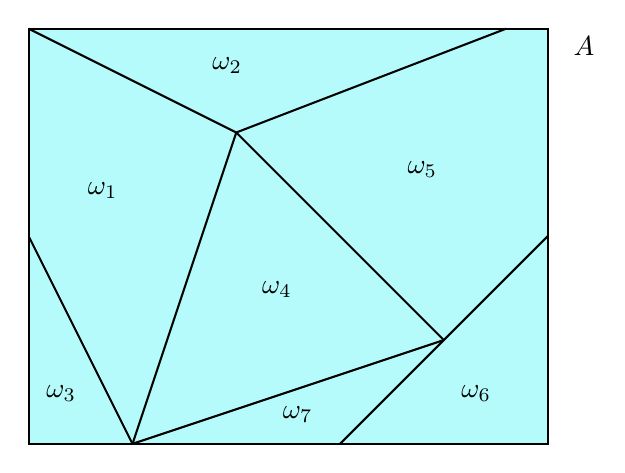
\begin{tikzpicture}[x=0.75pt,y=0.75pt,yscale=-1,xscale=1]
			%uncomment if require: \path (0,300); %set diagram left start at 0, and has height of 300
			
			%Shape: Rectangle [id:dp43293331661725487] 
			\draw  [fill={rgb, 61:red, 26; green, 120; blue, 120 }  ,fill opacity=0.5 ] (0,0) -- (250,0) -- (250,200) -- (0,200) -- cycle ;
			%Straight Lines [id:da5316126969281758] 
			\draw    (0,0) -- (100,50) ;
			%Straight Lines [id:da3315870854327041] 
			\draw    (100,50) -- (230,0) ;
			%Straight Lines [id:da34996079375608935] 
			\draw    (100,50) -- (200,150) ;
			%Straight Lines [id:da8348763175123195] 
			\draw    (250,100) -- (150,200) ;
			%Straight Lines [id:da06795938190747708] 
			\draw    (100,50) -- (50,200) ;
			%Straight Lines [id:da5655408089979519] 
			\draw    (0,100) -- (50,200) ;
			%Straight Lines [id:da12814303231022994] 
			\draw    (50,200) -- (200,150) ;
			
			% Text Node
			\draw (27,72.4) node [anchor=north west][inner sep=0.75pt]    {$\omega _{1}$};
			% Text Node
			\draw (87,12.4) node [anchor=north west][inner sep=0.75pt]    {$\omega _{2}$};
			% Text Node
			\draw (7,170.4) node [anchor=north west][inner sep=0.75pt]    {$\omega _{3}$};
			% Text Node
			\draw (111,120.4) node [anchor=north west][inner sep=0.75pt]    {$\omega _{4}$};
			% Text Node
			\draw (181,62.4) node [anchor=north west][inner sep=0.75pt]    {$\omega _{5}$};
			% Text Node
			\draw (207,170.4) node [anchor=north west][inner sep=0.75pt]    {$\omega _{6}$};
			% Text Node
			\draw (121,180.4) node [anchor=north west][inner sep=0.75pt]    {$\omega _{7}$};
			% Text Node
			\draw (261,2.4) node [anchor=north west][inner sep=0.75pt]    {$A$};
			
			
		\end{tikzpicture}
		
	\end{figure}
\end{frame}
\begin{frame}
	\begin{exercise}
		Demuestre que dado un conjunto $ A $, $ \Omega =\mpow{A} $ no es una partición de $ A $.
	\end{exercise}
\end{frame}
\begin{frame}
	
\end{frame}
\begin{frame}
	\begin{exercise}
		Demuestre que dado un conjunto $ A $ y $ \Omega\subsetneq\mpow{A} $ una partición, $ \abs{\Omega} = 1 $ si y solo si $ \Omega =\set{A} $.
	\end{exercise}
\end{frame}
\begin{frame}
	
\end{frame}
\begin{frame}
	\begin{exercise}
		Sea $ A $ un conjunto y $ B\subsetneq A $. Demuestre que $ \Omega =\set{B, A\setminus B} $ es una partición.
	\end{exercise}
\end{frame}
\begin{frame}
	
\end{frame}
\begin{frame}{Representante}
	\only{
		Usando otra vez el ejemplo de las filas. Sabemos que en cada fila hay una persona que está al frente de esta. A esta persona la podemos usar para identificar a la fila entera.
	}<1>
	\only{
		Ya en clases de equivalencia en general, podemos elegir un elemento de cada clase que identifique a su clase entera. A este elemento se le denomina \emph{representante de la clase}.	
	}<2>
\end{frame}
\begin{frame}{Representante de una clase}
	\begin{mdefinition}[Representante]
		Sea $ A $ un conjunto y $ \sim\subseteq A^{2} $ una relación de equivalencia. Para cada clase $ C $, se elige un elemento único el cual se denominará \emph{representante} de $ C $. Al conjunto de todos los representantes de las clases se le denotará por $ \tilde{R} $.
	\end{mdefinition}
\end{frame}
\begin{frame}
	\begin{exercise}
		Dada la relación de equivalencia de fracciones equivalentes. Demuestre que los $ (a, b)\in\nmath[2] $ tales que $ \mmcd{a, b} = 1 $ son elementos representantes.
	\end{exercise}
\end{frame}
\begin{frame}
	
\end{frame}
\begin{frame}
	\begin{exercise}
		Dada la relación de equivalencia de módulos. Demuestre que $ \tilde{R} =\set{0, 1, 2,\dotsc, n - 1} $ es un conjunto de representantes.
	\end{exercise}
\end{frame}
\begin{frame}
	
\end{frame}